\documentclass[10pt,fleqn]{article}
%\usepackage{graphicx}


\setlength{\topmargin}{-.75in}
\addtolength{\textheight}{2.00in}
\setlength{\oddsidemargin}{.00in}
\addtolength{\textwidth}{.75in}

\title{Math 4610 Lecture Notes \\
            \ \\
       A Brief Introduction to Github Usage
  \footnote{These notes are part of an Open Resource Educational project
            sponsored by Utah State University}}

\author{Joe Koebbe}

\nofiles

\pagestyle{empty}

\setlength{\parindent}{0in}

% new math commands


\setlength{\oddsidemargin}{-0.25in}
\setlength{\evensidemargin}{-0.25in}
\setlength{\textwidth}{6.75in}
\setlength{\headheight}{0.0in}
\setlength{\topmargin}{-0.25in}
\setlength{\textheight}{9.00in}

\makeindex

\usepackage{mathrsfs}

%\usepackage[pdftex]{graphicx}
\usepackage{epstopdf}

\newcounter{beans}

\newcommand{\ds}{\displaystyle}
\newcommand{\limit}[2]{\displaystyle\lim_{#1\to#2}}

\newcommand{\binomial}[2]{\ \left( \begin{array}{c}
                                  #1 \\
                                  #2
                                 \end{array}
                            \right) \
                         }
\newcommand{\ExampleRule}[2]
  {
  \noindent
  \rule{\linewidth}{1pt}
  \begin{example}
    #1
    \label{#2}
  \end{example}
  \rule{\linewidth}{1pt}
  \vskip0.125in
  }

\newcommand{\defbox}[1]
  {
   \ \\
   \noindent
   \setlength\fboxrule{1pt}
   \fbox{
        \begin{minipage}{6.5in}
          #1
        \end{minipage}
        }
   \ \\
  }
\newcommand{\verysmallworkbox}[1]
  {
   \ \\
   \noindent
   \setlength\fboxrule{1pt}
   \fbox{
        \begin{minipage}{6.5in}
           #1
           \ \\
           \vskip0.5in \ \\
           \ \\
        \end{minipage}
        }
   \ \\
  }
\newcommand{\smallworkbox}[1]
  {
   \ \\
   \noindent
   \setlength\fboxrule{1pt}
   \fbox{
        \begin{minipage}{6.5in}
           #1
           \ \\
           \vskip2.5in \ \\
           \ \\
        \end{minipage}
        }
   \ \\
  }
\newcommand{\halfworkbox}[1]
  {
   \ \\
   \noindent
   \setlength\fboxrule{1pt}
   \fbox{
        \begin{minipage}{6.5in}
           #1 \hfill
           \ \\
           \vskip3.25in \ \\
           \ \\
        \end{minipage}
        }
   \ \\
  }
\newcommand{\largeworkbox}[1]
  {
   \ \\
   \noindent
   \setlength\fboxrule{1pt}
   \fbox{
        \begin{minipage}{6.5in}
           #1
           \ \\
           \vskip7.5in \ \\
           \ \\
        \end{minipage}
        }
   \ \\
  }
\newcommand{\flexworkbox}[2]
  {
   \ \\
   \noindent
   \setlength\fboxrule{1pt}
   \fbox{
        \begin{minipage}{6.5in}
           #1
           \ \\

           \vskip#2 \ \\
           \ \\
        \end{minipage}
        }
   \ \\
  }


% symbols for sets of numbers

\newcommand{\natnumb}{$\cal N$}
\newcommand{\whonumb}{$\cal W$}
\newcommand{\intnumb}{$\cal Z$}
\newcommand{\ratnumb}{$\cal Q$}
\newcommand{\irrnumb}{$\cal I$}
\newcommand{\realnumb}{$\cal R$}
\newcommand{\cmplxnumb}{$\cal C$}

% misc. commands

\newcommand{\mma}{{\it Mathematica}}
\newcommand{\sech}{\mbox{ sech}}
 
\newtheorem{theorem}{Theorem}
\newtheorem{example}{Example}
\newtheorem{definition}{Definition}
\newtheorem{problem}{Problem}

\setcounter{secnumdepth}{2}
\setcounter{tocdepth}{4}


\begin{document}
\maketitle
\newpage
%%%%%%%%%%%%%%%%%%%%%%%%%%%%%%%%%%%%%%%%%%%%%%%%%%%%%%%%%%%%%%%%%%%%%%%%%%%%%%%%
%%%%%%%%%%%%%%%%%%%%%%%%%%%%%%%%%%%%%%%%%%%%%%%%%%%%%%%%%%%%%%%%%%%%%%%%%%%%%%%%

%%%%%%%%%%%%%%%%%%%%%%%%%%%%%%%%%%%%%%%%%%%%%%%%%%%%%%%%%%%%%%%%%%%%%%%%%%%%%%%%
%%%%%%%%%%%%%%%%%%%%%%%%%%%%%%%%%%%%%%%%%%%%%%%%%%%%%%%%%%%%%%%%%%%%%%%%%%%%%%%%
\vskip0.1in\hrule\vskip0.1in
\noindent
{\bf Github Primer for Math 4610 at USU: Get an Account} 
\vskip0.1in\hrule\vskip0.1in
\noindent
To create an account on GitHub, go to the Github site
\begin{verbatim}

    https://github.com

\end{verbatim}
This site will display a place to create an account or sign in to an existin
account.
\vskip0.1in\hrule\vskip0.1in
\vfill
\begin{figure}[h]
\centering
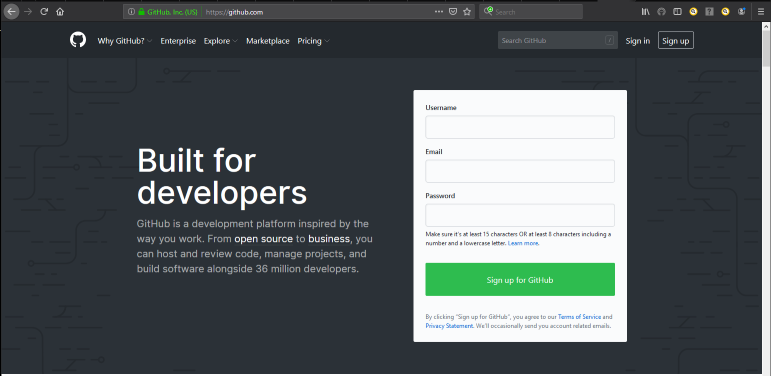
\includegraphics{../images/github_01.png}
\vskip0.1in
\caption{{Screenshot} taken using {\bf Snip \& Sketch}. This is an app on
         my Windows 10 box}
\end{figure}
\eject
%%%%%%%%%%%%%%%%%%%%%%%%%%%%%%%%%%%%%%%%%%%%%%%%%%%%%%%%%%%%%%%%%%%%%%%%%%%%%%%%
%%%%%%%%%%%%%%%%%%%%%%%%%%%%%%%%%%%%%%%%%%%%%%%%%%%%%%%%%%%%%%%%%%%%%%%%%%%%%%%%
\vskip0.1in\hrule\vskip0.1in
\noindent
{{\bf GitHub Primer for Math 4610 at USU:} Setting up a Repository} 
\vskip0.1in\hrule\vskip0.1in
\noindent
Once you log in, you will need to build a repository for use in the class and
to turn in homework and completed tasks and projects. For the course, you will
create a repository named the following:
\begin{verbatim}

    math4610

\end{verbatim}
Use only the characters above and using the following rules:
\begin{enumerate}
  \item Use only lower case characters - github is case senesitive.
  \item Do not put any blanks in the name of the repository.
\end{enumerate}
Note that the instructor will use only this repository name in looking for your
work.
\vskip0.1in\hrule\vskip0.1in
\vfill
\begin{figure}[h]
\centering
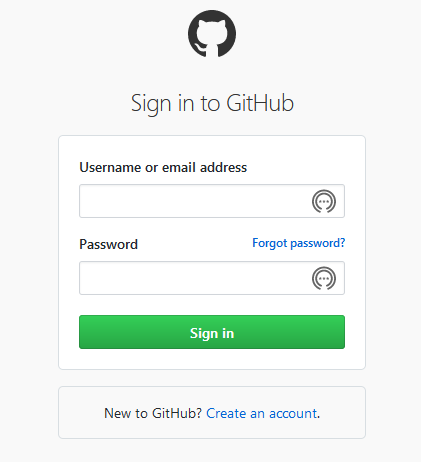
\includegraphics{../images/github_02.png}
\caption{{Screenshot} taken using {\bf Snip \& Sketch}. This is an app on
         my Windows 10 box}
\end{figure}
\eject
%%%%%%%%%%%%%%%%%%%%%%%%%%%%%%%%%%%%%%%%%%%%%%%%%%%%%%%%%%%%%%%%%%%%%%%%%%%%%%%%
%%%%%%%%%%%%%%%%%%%%%%%%%%%%%%%%%%%%%%%%%%%%%%%%%%%%%%%%%%%%%%%%%%%%%%%%%%%%%%%%
\vskip0.1in\hrule\vskip0.1in
\noindent
{{\bf Github Primer for Math 4610 at USU:} List the Contents of the Home
    Directory} 
\vskip0.1in\hrule\vskip0.1in
\noindent
If you have an account on GitHub, you will already know a lot about these
things. However, when you are logged in you will see the main screen with any
repositories you may already have created. We will go through the steps to
build and name repositories in the next few pages.

\vskip0.1in\hrule\vskip0.1in
\vfill
\begin{figure}[h]
\centering
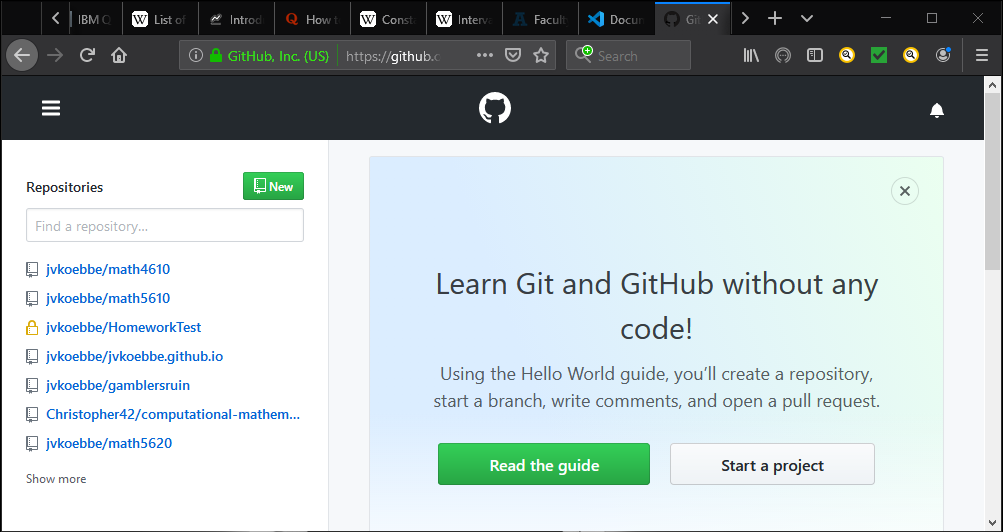
\includegraphics{../images/github_03.png}
\caption{{Screenshot} taken using {\bf Snip \& Sketch}. This is an app on
         my Windows 10 box}
\end{figure}
\eject
%%%%%%%%%%%%%%%%%%%%%%%%%%%%%%%%%%%%%%%%%%%%%%%%%%%%%%%%%%%%%%%%%%%%%%%%%%%%%%%%
%%%%%%%%%%%%%%%%%%%%%%%%%%%%%%%%%%%%%%%%%%%%%%%%%%%%%%%%%%%%%%%%%%%%%%%%%%%%%%%%
\end{document}
